% Created 2018-04-04 Wed 11:13
% Intended LaTeX compiler: pdflatex
\documentclass[presetation]{beamer}
\usepackage[utf8]{inputenc}
\usepackage[T1]{fontenc}
\usepackage{graphicx}
\usepackage{grffile}
\usepackage{longtable}
\usepackage{wrapfig}
\usepackage{rotating}
\usepackage[normalem]{ulem}
\usepackage{amsmath}
\usepackage{textcomp}
\usepackage{amssymb}
\usepackage{capt-of}
\usepackage{hyperref}
\usetheme{Madrid}
\author{Evan Misshula}
\date{2018-03-28}
\title{Why teaching functional programming to undergraduates at CUNY is important}
\hypersetup{
 pdfauthor={Evan Misshula},
 pdftitle={Why teaching functional programming to undergraduates at CUNY is important},
 pdfkeywords={},
 pdfsubject={},
 pdfcreator={Emacs 25.2.1 (Org mode 9.0.6)}, 
 pdflang={English}}
\begin{document}

\maketitle

\begin{frame}[label={sec:org86111c2}]{Plan for the talk}
\begin{enumerate}
\item Why Functional Programming is intellectually interesting
\end{enumerate}
\pause   
(particularly with Haskell)
\pause
\begin{enumerate}
\item The size and growth of the Tech sector in NYC
\item The size, growth and earnings of CUNY CS grads
\item The demographic biasis of the Tech Industry relative to NYC Population
\item My thoughts on how helping to close this gap can benefit you and
your employer
\end{enumerate}
\end{frame}


\begin{frame}[label={sec:org559d467}]{First computers were imperative by necessity}
\begin{center}
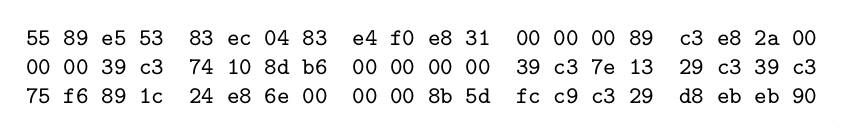
\includegraphics[width=.9\linewidth]{./images/machineCode.png}
\end{center}
\end{frame}

\begin{frame}[label={sec:orgc7373ce}]{Programming languages help us think}
\begin{center}
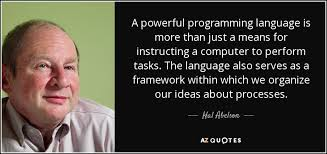
\includegraphics[width=.9\linewidth]{./images/lang.jpeg}
\end{center}
\end{frame}

\begin{frame}[label={sec:orga9a6de2}]{Languages encourage patterns of thought}
\begin{center}
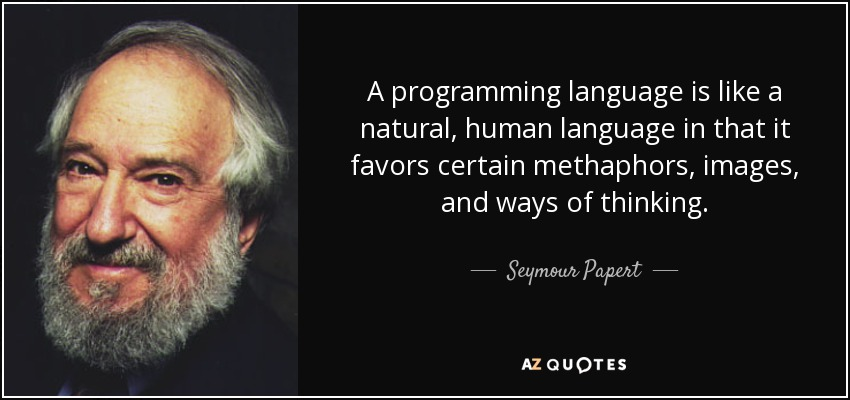
\includegraphics[width=.9\linewidth]{./images/papert.jpeg}
\end{center}
\end{frame}

\begin{frame}[label={sec:org7075503}]{There are dissenting opinions}
\begin{center}
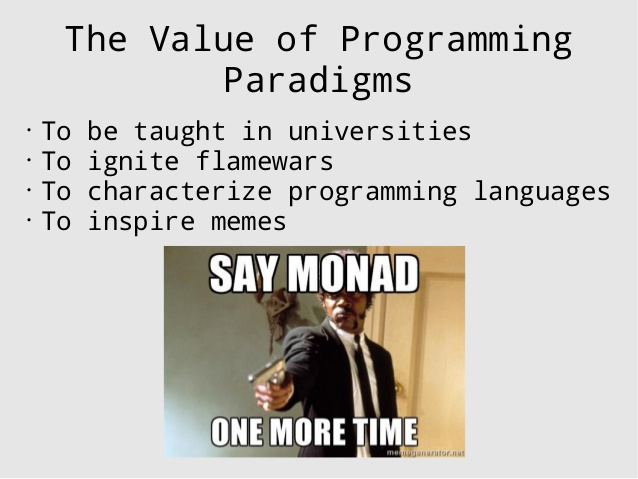
\includegraphics[width=.9\linewidth]{./images/noVal.jpg}
\end{center}
\begin{itemize}
\item Vsevolod Dyomkin \href{https://www.slideshare.net/vseloved/can-functional-programming-be-liberated-from-static-typing}{published October 31, 2015}
\end{itemize}
\end{frame}


\begin{frame}[fragile,label={sec:org544e3bc}]{Counterexamples of good languages}
 \begin{center}
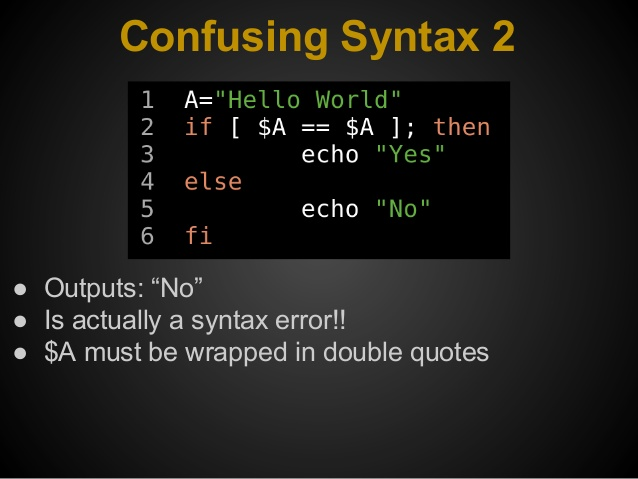
\includegraphics[width=.6\linewidth]{./images/bashHorror.jpeg}
\end{center}
\pause
\begin{itemize}
\item actually the slide is wrong
\end{itemize}
\pause
\begin{itemize}
\item comparison should be \texttt{[[}
\end{itemize}
\end{frame}


\begin{frame}[fragile,label={sec:org1743c69}]{You can't talk about poor language design and not mention JS}
 \begin{verbatim}
console.log(0.1 + 0.2);
console.log(0.1 + 0.2 == 0.3);
\end{verbatim}
\pause
\begin{itemize}
\item 0.30000000000000004
\item false
\end{itemize}
\end{frame}



\begin{frame}[fragile,label={sec:org6347cf8}]{Comparisons can fail}
 \begin{verbatim}
console.log(1 < 2 < 3);
console.log(3 > 2 > 1);
\end{verbatim}
\pause
\begin{itemize}
\item true (1<2) -> true is implicitly coerced to 1 and 1<3
\item false (3>2) -> true coerced to 1 and and 1>1 is false
\end{itemize}
\end{frame}

\begin{frame}[fragile,label={sec:org960434e}]{Even assignment is perilous}
 \begin{verbatim}
var a= [1,2,3];
a[10]=99;
console.log(a[10])
console.log(a[6])
\end{verbatim}
\pause
\begin{itemize}
\item 99
\item\relax [1, 2, 3, <7 empty items>, 99]
\end{itemize}
\end{frame}

\begin{frame}[label={sec:org2a20c0a}]{Yet Haskell allows us to}
\pause
\begin{itemize}
\item Explore recursion both in functions and in data structures
\end{itemize}
\pause
\begin{itemize}
\item Rewrite classic sort algorithms in breathtakingly simple form
\end{itemize}
\pause
\begin{itemize}
\item Introduce students to algebraic ideas on functions so that they can
master abstraction
\end{itemize}
\end{frame}

\begin{frame}[label={sec:org34e7716}]{Right triangle problem}
\begin{block}{Let's find a problem that puts constraints on tuples}
\begin{itemize}
\item Which right triangle that has integers for all sides and all sides
equal to or smaller than 10 has a perimeter of 24?
\end{itemize}
\pause 
\begin{itemize}
\item crack the problem like an egg
\end{itemize}
\pause
\begin{itemize}
\item Opportunity to teach: \alert{solution by problem relaxation}
\end{itemize}
\end{block}
\end{frame}
\begin{frame}[fragile,label={sec:org485f41e}]{Right triangle problem relax solution}
 \begin{block}{Integer sides all < 10 and perimeter = 24}
\begin{itemize}
\item generate all tuples of sides less than 10
\end{itemize}
\pause
\begin{itemize}
\item designate z as the hypotenuse (bigger than x and y)
\end{itemize}
\pause
\begin{itemize}
\item make \(x^2 + y^2 = z^2\)
\end{itemize}
\begin{verbatim}
:set +m
length([(x,y,z) | x<-[1..10],y<-[1..10],
	z<-[1..10],y<z,x<z,
	(x^2 + y^2 == z^2)])
i==i
\end{verbatim}

\begin{verbatim}

Prelude Control.Applicative| Prelude Control.Applicative| 4
\end{verbatim}
\end{block}
\end{frame}


\begin{frame}[fragile,label={sec:org4393f83}]{Adding the perimeter constraint}
 \begin{block}{Let's add constraints}
\begin{itemize}
\item the perimeter equal 24
\item \(a + b + c = 24\)
\end{itemize}

\begin{verbatim}
:set +m

length([(x,y,z) | x<-[1..10],y<-[1..10],z<-[1..10],
	y<z,
	x+y+z==24,
	(x^2 + y^2 == z^2)])
[(x,y,z) | x<-[1..10],y<-[1..10],z<-[1..10],y<z,
  x+y+z==24,
  (x^2 + y^2 == z^2)]
i==i
\end{verbatim}

\begin{verbatim}

Prelude Control.Applicative> Prelude Control.Applicative| Prelude Control.Applicative| Prelude Control.Applicative| 2
Prelude Control.Applicative| Prelude Control.Applicative| [(6,8,10),(8,6,10)]
\end{verbatim}
\end{block}
\end{frame}

\begin{frame}[fragile,label={sec:org9c43f74}]{Type system}
 \begin{block}{Haskell is statically typed}
\begin{itemize}
\item Haskell allows students inquire about the type
\begin{itemize}
\item We can see that type by using the ':t' command in the repl:
\end{itemize}
\end{itemize}
\begin{verbatim}
 :t 'a'
 :t True
 :t "HELLO!"
 :t (True, 'a')
 :t 4 == 5
1==1
\end{verbatim}

\begin{verbatim}
'a' :: Char
True :: Bool
"HELLO!" :: [Char]
(True, 'a') :: (Bool, Char)
4 == 5 :: Bool
\end{verbatim}
\end{block}

\begin{block}{Haskell has functions that work on different types}
\pause
\begin{itemize}
\item These are polymorphic functions
\begin{itemize}
\item examples
\end{itemize}
\end{itemize}
\begin{verbatim}
head [1,2,3]
head "Evan"
fst ("Evan","Misshula")
snd (1,3)
1==1
\end{verbatim}

\begin{verbatim}
1
'E'
Evan
3
\end{verbatim}
\end{block}
\end{frame}

\begin{frame}[label={sec:org1945b97}]{Decompose the typeclass}
\begin{block}{(==) :: Eq a => a -> a -> Bool}
\begin{itemize}
\item Typeclass constraint 
\begin{itemize}
\item The declaration we can read says:
\end{itemize}
\end{itemize}
\pause     
\begin{itemize}
\item The equality function takes two variables of the same type and returns a Bool
\end{itemize}
\pause 
\begin{itemize}
\item The new part 'Eq a =>' says:
\item The type must be part of Eq typeclass
\begin{itemize}
\item This is called the class constraint
\end{itemize}
\end{itemize}
\end{block}
\end{frame}
\begin{frame}[fragile,label={sec:orge5cc17d}]{Interface of Eq}
 \begin{block}{The Eq typeclass provides an interface for testing for equality}
\begin{itemize}
\item Eq is used for types that support equality testing
\begin{itemize}
\item Its members implement both:
\begin{itemize}
\item '=='
\item '/='
\end{itemize}
\end{itemize}
\end{itemize}
\begin{verbatim}
5==5
5/=5
'a' == 'a'
"Ho Ha" == "Ho Ha"
3.4 == 3.4
  1==1
\end{verbatim}

\begin{verbatim}
True
False
True
True
True
\end{verbatim}
\end{block}
\end{frame}


\begin{frame}[fragile,label={sec:org3cad51b}]{Introducing Ord typeclass}
 \begin{block}{Ord is for types that have an ordering}
\begin{itemize}
\item We can see the type of '>' comparison
\item We can see some functions which rely on being in the ord typeclass
\end{itemize}
\begin{verbatim}
:t (>)
"Abc"< "Zev"
compare "Abc" "Zev"
5 >= 2
compare 5 3
1==1
\end{verbatim}

\begin{verbatim}
(>) :: Ord a => a -> a -> Bool
True
LT
True
GT
\end{verbatim}
\end{block}
\end{frame}


\begin{frame}[label={sec:org43cf92d}]{Ord has a connection with inference}
\begin{block}{Ord is important in statistics}
\begin{itemize}
\item Ord can be used to explain: \alert{ordinal levels of measurement}
\end{itemize}
\pause
\begin{itemize}
\item Ord can also be used to introduce: \alert{utility curves}
\end{itemize}
\end{block}
\end{frame}


\begin{frame}[fragile,label={sec:org29b26b6}]{Introducing Show typeclass}
 \begin{block}{Everything except function has been part of show}
\begin{itemize}
\item It works like Java or Ruby's toString methods
\item Mostly we use it to examine a value
\end{itemize}
\begin{verbatim}
show 3
show 5.334
show True
1==1
\end{verbatim}

\begin{verbatim}
3
5.334
True
\end{verbatim}
\end{block}
\end{frame}


\begin{frame}[fragile,label={sec:org7472a15}]{Introducing Read typeclass}
 \begin{block}{Read is the inverse of show}
\begin{itemize}
\item It works reads a string and returns a type which supports the interface Read
\end{itemize}
\pause
\begin{itemize}
\item You can use it to create Javascript like craziness
\end{itemize}
\pause
\begin{itemize}
\item \alert{But you have to work at it}
\end{itemize}
\begin{verbatim}
read "True" || False                          
read "8.2" + 3.8                                    
read "5" - 2         
read "[1,2,3,4]" ++ [3]
1==1
\end{verbatim}

\begin{verbatim}
True
12.0
3
[1,2,3,4,3]
\end{verbatim}
\end{block}
\end{frame}

\begin{frame}[fragile,label={sec:org2d1d835}]{Limits to the type inference system}
 \begin{block}{Let's look at a type error}
\begin{verbatim}
read 4
1==1
\end{verbatim}

\begin{verbatim}
<interactive>:2327:6: error:
    • Could not deduce (Num String) arising from the literal ‘4’
      from the context: Read a
        bound by the inferred type of it :: Read a => a
        at <interactive>:2327:1-6
    • In the first argument of ‘read’, namely ‘4’
      In the expression: read 4
      In an equation for ‘it’: it = read 4
\end{verbatim}

\begin{itemize}
\item GHCI is saying it does not know what type to return
\begin{itemize}
\item Do you want an Float or an Integer?
\end{itemize}
\end{itemize}
\end{block}
\end{frame}

\begin{frame}[fragile,label={sec:orgd8972ab}]{Type specification}
 \begin{block}{We can specify a type}
\begin{itemize}
\item We just add '::<Type>' and read will work
\end{itemize}
\begin{verbatim}
read "5" :: Int
read "5" :: Float
(read "5" :: Int) * 4
read "[1,2,3,4]" :: [Int]
read "(3,'a')" :: (Int, Char)
1==1
\end{verbatim}

\begin{verbatim}
5
5.0
20
[1,2,3,4]
(3,'a')
\end{verbatim}
\end{block}
\end{frame}

\begin{frame}[fragile,label={sec:org41be4d2}]{Enum type class}
 \begin{block}{Sequentially ordered types}
\begin{itemize}
\item Being \emph{sequentialy ordered} means that they can be counted in order
\item This property is also called being \emph{enumerable}
\item We can use them in list ranges
\begin{itemize}
\item they each have a predecessor which you can get with 'pred'
\item they each have a successor which you can get with 'succ'
\end{itemize}
\end{itemize}
\begin{verbatim}
['a'..'e']
[LT .. GT]
[3..7]
succ 'B'
1==1
\end{verbatim}

\begin{verbatim}
abcde
[LT,EQ,GT]
[3,4,5,6,7]
'C'
\end{verbatim}
\end{block}
\end{frame}

\begin{frame}[fragile,label={sec:org405c526}]{Bounded Type class}
 \begin{block}{Bounded type class has concrete types}
\begin{itemize}
\item with maximum and minimum elements
\begin{itemize}
\item minBound and maxBound are functions with polymorphic type
\begin{itemize}
\item (Bounded a) => a
\end{itemize}
\end{itemize}
\end{itemize}
\begin{verbatim}
minBound :: Int
maxBound :: Char
maxBound :: Bool
minBound :: Bool
i==i
\end{verbatim}

\begin{verbatim}
-9223372036854775808
'\1114111'
True
False
\end{verbatim}
\end{block}
\end{frame}

\begin{frame}[fragile,label={sec:org34ee6a4}]{Numeric Types}
 \begin{block}{Numeric types can be operated on mathematically}
\begin{itemize}
\item Let's look at this type
\end{itemize}
\begin{verbatim}
:t (*)
(5 :: Int) * (6 :: Integer)
(5 :: Int) * 6
i==i
\end{verbatim}

\begin{verbatim}
(*) :: Num a => a -> a -> a
<interactive>:2350:15: error:
    • Couldn't match expected type ‘Int’ with actual type ‘Integer’
    • In the second argument of ‘(*)’, namely ‘(6 :: Integer)’
      In the expression: (5 :: Int) * (6 :: Integer)
      In an equation for ‘it’: it = (5 :: Int) * (6 :: Integer)
30
\end{verbatim}
\end{block}
\end{frame}

\begin{frame}[fragile,label={sec:org729c9c8}]{Integral and Floating types}
 \begin{block}{Integral and Floating types}
\begin{itemize}
\item The Integral typeclass only includes Integer and Int
\item The Floating typeclass only includes floats and double
\end{itemize}
\begin{verbatim}
:t fromIntegral
fromIntegral (length [1,2,3,4]) + 3.2
i==i
\end{verbatim}

\begin{verbatim}
fromIntegral :: (Num b, Integral a) => a -> b
7.2
\end{verbatim}
\end{block}
\end{frame}


\begin{frame}[fragile,label={sec:org791ccad}]{Curried Functions}
 \begin{block}{Every function in haskell only takes one argument}
\begin{itemize}
\item But what about  'max' or min?
\item We actually apply parameters to functions one at time
\begin{itemize}
\item These are called "curried" functions
\begin{itemize}
\item This is after Haskell Curry
\item[{max}] (Ord a) => a -> a -> a
\item[{max}] (Ord a) => a -> (a -> a)
\end{itemize}
\end{itemize}
\item If we call a function with to few parameters we get back a partially
applied function
\end{itemize}
\begin{verbatim}
:set +m

-- multThree :: (Num a) => a -> a -> a -> a  
multThree x y z = x * y * z  
multThree 3 5 9 ==  ((multThree 3) 5) 9
i==1
\end{verbatim}

\begin{verbatim}

Prelude Control.Applicative> Prelude Control.Applicative> Prelude Control.Applicative> True
\end{verbatim}
\end{block}
\end{frame}

\begin{frame}[fragile,label={sec:orgfb11fa3}]{Curried comparison}
 \begin{block}{Here is a curried comparison}
\begin{itemize}
\item These are the same because 'x' is on both sides of the equation
\end{itemize}
\begin{verbatim}
-- compareWithHundred :: (Num a, Ord a, Show a) => a -> Ordering  
compareWithHundred x = compare 100 x  

-- compareWithHundred1 :: (Num a, Ord a, Show a) => a -> Ordering  
compareWithHundred1 = compare 100  
\end{verbatim}
\end{block}
\end{frame}

\begin{frame}[fragile,label={sec:orgfd64a4d}]{Example partial application}
 \begin{block}{Let's look at an infix function}
\begin{itemize}
\item simply surround the function with parentheses and only supply one of
the parameters
\item this is called 'sectioning'
\end{itemize}
\begin{verbatim}
-- divideByTen :: (Floating a) => a -> a
divideByTen = (/10)
\end{verbatim}
\end{block}
\end{frame}

\begin{frame}[fragile,label={sec:org975fc72}]{partial application of a string function}
 \begin{block}{String functions can be partially applied too}
\begin{itemize}
\item this is written in point free style
\item it is also sectioned
\end{itemize}
\begin{verbatim}
-- isUpperAlphanum :: Char -> Bool
isUpperAlphanum = (`elem` ['A'..'Z'])
\end{verbatim}
\end{block}
\end{frame}


\begin{frame}[fragile,label={sec:orgdff85db}]{Returned functions}
 \begin{block}{Functions can return functions}
\begin{itemize}
\item take a function and apply it twice
\end{itemize}
\begin{verbatim}
-- applyTwice :: (a -> a) -> a -> a
applyTwice f x = f (f x)
\end{verbatim}
\end{block}
\end{frame}

\begin{frame}[fragile,label={sec:org4f101ee}]{ZipWith}
 \begin{block}{We are going to implement ZipWith}
\begin{itemize}
\item It joins two lists and performs a function on the corresponding elements
\end{itemize}
\begin{verbatim}
-- zipWith' :: (a -> b -> c) -> [a] -> [b] -> [c]
zipWith' _ [] _ = []
zipWith' _ _ [] = []
zipWith' f (x:xs) (y:ys) = f x y : zipWith' f xs ys
\end{verbatim}
\end{block}
\end{frame}

\begin{frame}[fragile,label={sec:org05453c1}]{flip}
 \begin{block}{flip changes the order of the arguements}
\begin{verbatim}
-- flip' :: (a -> b -> c) -> (b -> a -> c)
flip' f = g
    where g x y = f y x

-- flip'' :: (a -> b -> c) -> b -> a -> c
flip'' f y x = f x y
\end{verbatim}
\end{block}
\end{frame}

\begin{frame}[fragile,label={sec:orgced0ebc}]{Maps and Filters}
 \begin{block}{Map}
\begin{itemize}
\item map takes a function applies the function to each element of a list
\end{itemize}
\begin{verbatim}
-- map :: (a -> b) -> [a] -> [b]
map _ [] = []
map f (x:xs) = f x : map f xs
\end{verbatim}
\end{block}
\end{frame}

\begin{frame}[fragile,label={sec:org2c3db7f}]{Filter}
 \begin{block}{Filter}
\begin{itemize}
\item 'filter' take a function called a predicate and a list of any type
\item the predicate takes an element of the list and returns a Bool
\begin{itemize}
\item the filter returns elements for which the predicate is True
\end{itemize}
\end{itemize}
\begin{verbatim}
filter :: (a -> Bool) -> [a] -> [a]
filter _ [] = []
filter p (x:xs) 
    | p x       = x : filter p xs
    | otherwise = filter p xs
\end{verbatim}
\end{block}
\end{frame}

\begin{frame}[label={sec:orgc694baa}]{Lambdas}
\begin{block}{Lamdas are anonymous functions}
\begin{itemize}
\item These are unnamed functions
\item They are passed as parameters to other functions
\item They work like composition in math
\item They are called 'lambdas' because of the 'lambda calculus'
\end{itemize}
\end{block}
\end{frame}

\begin{frame}[label={sec:org93e2729}]{Church and Turing}
\begin{center}
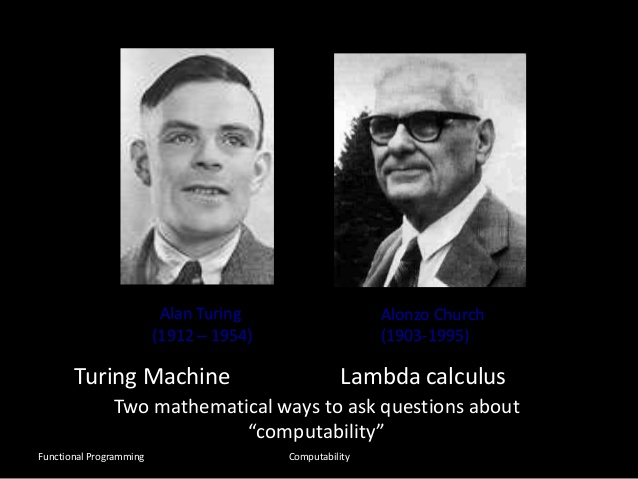
\includegraphics[width=.9\linewidth]{images/computability.jpg}
\end{center}
\end{frame}

\begin{frame}[label={sec:org03eeb7c}]{Lambda Calculus}
\begin{block}{Lambda Calculus is a formal system for computation}
\begin{itemize}
\item it is equivelent to calculation by Turing Machine
\item invented by Alonzo Church in the 1930's
\item Church was Turing's thesis advisor
\begin{itemize}
\item a function is denoted by the greek letter \(\lambda\)
\item a function f(x) that maps x -> f(x) is:
\begin{itemize}
\item \(\lambda x.y\)
\end{itemize}
\end{itemize}
\end{itemize}
\end{block}
\end{frame}
\begin{frame}[fragile,label={sec:org73ab9f1}]{Example of a lambda}
 \begin{block}{We can pass a lambda to ZipWith}
\begin{itemize}
\item a lambda function in Haskell starts with '$\backslash$'
\item can't define several parameters for one para,eters
\end{itemize}
\begin{verbatim}
zipWith (\a b -> (a * 30 + 3) / b) [5,4,3,2,1] [1,2,3,4,5]
1==1
\end{verbatim}
\end{block}
\end{frame}

\begin{frame}[fragile,label={sec:org87c1bc1}]{Quicksort}
 \begin{block}{specification}
\begin{verbatim}
-- quicksort :: (Ord a) => [a] -> [a]  
quicksort [] = []  
quicksort (x:xs) =   
    let smallerSorted = quicksort [a | a <- xs, a <= x]  
	biggerSorted = quicksort [a | a <- xs, a > x]  
    in  smallerSorted ++ [x] ++ biggerSorted  
1==1
\end{verbatim}
\end{block}
\end{frame}
\begin{frame}[fragile,label={sec:orgfd12325}]{Folds}
 \begin{block}{Folds encapsulate several functions with (x:xs) patterns}
\begin{itemize}
\item they reduce a list to a single value
\item 'foldl' is the left fold function
\end{itemize}
\begin{verbatim}
sum' :: (Num a) => [a] -> a
sum' xs = foldl (\acc x -> acc + x) 0 xs

sum'' :: (Num a) => [a] -> a
sum'' = foldl (+) 0
1==1
\end{verbatim}
\end{block}
\end{frame}

\begin{frame}[fragile,label={sec:org0147a91}]{Function application}
 \begin{block}{Function application with \$}
\begin{itemize}
\item '\$' is called the \emph{function application}
\item changes to right association
\item keeps us from writing parentheses
\end{itemize}

\begin{verbatim}
map ($ 3) [(4+), (10*), (^2), sqrt]
1==1
\end{verbatim}

\begin{verbatim}
[7.0,30.0,9.0,1.7320508075688772*** Exception: <interactive>:2394:1-29: Non-exhaustive patterns in function map
\end{verbatim}
\end{block}
\end{frame}

\begin{frame}[fragile,label={sec:org6498a44}]{Function composition}
 \begin{block}{Function composition is just like math}
\begin{itemize}
\item In math  \(f \centerdot g(x) = f(g(x))\)
\item Let's look at Haskell function
\item g takes a -> b
\item f takes b -> c
\end{itemize}
\pause
\begin{itemize}
\item so the composition take f . g takes a -> c
\end{itemize}
\begin{verbatim}
(.) :: (b -> c) -> (a -> b) -> a -> c
f . g = \x -> f (g x)
\end{verbatim}
\end{block}
\end{frame}

\begin{frame}[fragile,label={sec:org7ab8db7}]{Function composition examples}
 \begin{block}{Function composition examples}
\begin{itemize}
\item with a \(\lambda\)
\item with point free notation
\end{itemize}
\begin{verbatim}
map (\x -> negate (abs x)) [5,-3,-6,7,-3,2,-19,24]
map (negate . abs) [5,-3,-6,7,-3,2,-19,24]
\end{verbatim}

\begin{verbatim}
[-5,-3,-6,-7,-3,-2,-19,-24*** Exception: <interactive>:2394:1-29: Non-exhaustive patterns in function map
\end{verbatim}
\end{block}
\end{frame}

\section{Functors, Applicative Functors and Monoids}
\label{sec:org045cc1b}
\begin{frame}[label={sec:org01665b8}]{Polymorphism on a higher level}
\begin{itemize}
\item Types are not part of a hierarchy
\item We can think about how they should act
\begin{itemize}
\item then connect them with typeclasses
\end{itemize}
\end{itemize}
\end{frame}

\begin{frame}[label={sec:orgdc0e7a4}]{Functors defined}
\begin{columns}
\begin{column}{.48\columnwidth}
\begin{definition}[definition]
A functor is a typeclass for all the things that can be mapped over

\pause
\end{definition}
\end{column}
\begin{column}{.48\columnwidth}
\begin{definition}[Haskell syntax definition]
\begin{itemize}
\item class Functor f where
\begin{description}
\item[{fmap}] (a -> b) -> f a -> f b
\end{description}
\end{itemize}
\end{definition}
\end{column}
\end{columns}
\end{frame}


\begin{frame}[fragile,label={sec:org0d9148a}]{Analogy with other typeclasses}
 \begin{block}{Typeclasses define functions}
\begin{itemize}
\item Eq \emph{defines} concrete types that are equatable
\begin{itemize}
\item functions ('\texttt{=') and ('/}')
\end{itemize}
\item Ord \emph{defines} concrete types that 'orderabe'
\begin{itemize}
\item implements the 'compare' function
\end{itemize}
\item Enum \emph{defines} concrete types that enumerable
\begin{itemize}
\item defines '..' a range
\end{itemize}
\end{itemize}
\end{block}
\end{frame}

\begin{frame}[label={sec:org7e2fb16}]{List Functor examples}
\begin{example}[List Functor Examples]
\begin{itemize}
\item map:: (a -> b)  -> [a] -> [b]
\item instance Functor [] where
\begin{itemize}
\item fmap = map
\end{itemize}
\end{itemize}
\end{example}
\end{frame}


\begin{frame}[fragile,label={sec:orgeb6728d}]{Functor code in the repl}
 \begin{block}{List Functor in the repl}
\begin{verbatim}
  :t map
  fmap (*2) [1..3]
  map (*2) [1..3]
i==i
\end{verbatim}

\begin{verbatim}
map :: (t -> a) -> [t] -> [a]
[2,4,6]
[2,4,6*** Exception: <interactive>:2394:1-29: Non-exhaustive patterns in function map
\end{verbatim}
\end{block}
\end{frame}

\begin{frame}[fragile,label={sec:org29871be}]{Maybe Functor examples}
 \begin{example}[Maybe Functor Examples]
\begin{verbatim}
type myMaybe a = Nothing | Just a 

instance Functor myMaybe where
  fmap f (Just x) = Just (f x)
  fmap f Nothing = Nothing
\end{verbatim}
\end{example}
\end{frame}
\begin{frame}[fragile,label={sec:org150e448}]{Maybe Functor code in the repl}
 \begin{block}{Maybe Functor in the repl}
\begin{verbatim}
:t fmap
fmap (++ " HEY GUYS IM INSIDE THE JUST") (Just "Something serious.")
fmap (++ " HEY GUYS IM INSIDE THE JUST") Nothing
fmap (*2) (Just 200)
fmap (*2) Nothing
i==i
\end{verbatim}

\begin{verbatim}
fmap :: Functor f => (a -> b) -> f a -> f b
Just "Something serious. HEY GUYS IM INSIDE THE JUST"
Nothing
Just 400
Nothing
\end{verbatim}
\end{block}
\end{frame}



\section{Functor Laws}
\label{sec:orgdd55417}
\begin{frame}[label={sec:org3a5933c}]{Functor Law intuition}
\begin{block}{If functors mean that something can be mapped over\ldots{}}
\begin{itemize}
\item then calling 'fmap' on a functor should
\begin{itemize}
\item map a function over the functor
\end{itemize}
\end{itemize}
\pause
\begin{itemize}
\item \alert{Nothng else}
\end{itemize}
\end{block}
\end{frame}

\begin{frame}[label={sec:orgf2e4a5d}]{The First Functor Laws}
\begin{definition}[The First Functor Law]
states that if we map the identity (id) function over a functor, we
get the functor
\begin{itemize}
\item fmap id = id
\end{itemize}
\end{definition}
\end{frame}

\begin{frame}[fragile,label={sec:org421eaf9}]{Identity in the Repl}
 \begin{block}{Identity functions in the repl}
\begin{verbatim}
fmap id (Just 3)
id (Just 3)
fmap id [1..5]
id [1..5]
fmap id []
fmap id Nothing
1==1
\end{verbatim}

\begin{verbatim}
Just 3
Just 3
[1,2,3,4,5]
[1,2,3,4,5]
[]
Nothing
\end{verbatim}
\end{block}
\end{frame}

\begin{frame}[label={sec:org19db90a}]{The Second Functor Law}
\begin{definition}[The Second Functor Law says]
The Second Functor Law says that composing two functions and then
mapping the composed function over a functor is the same as first
mapping one function over the functor and then mapping the other one.
\begin{itemize}
\item fmap (f.g) = fmap f . fmap g
\item fmap (f.g) F = fmap f (fmap g F)
\end{itemize}
\end{definition}
\end{frame}

\begin{frame}[fragile,label={sec:org2565e11}]{Composition in the Repl}
 \begin{block}{Composition functions in the repl}
\begin{verbatim}
fmap ((+1).(*2)) (Just 3)
fmap (+1) (fmap (*2) (Just 3))
fmap  ((+1).(*2)) [1..5]
fmap (+1) (fmap (*2) [1..5])
1==1
\end{verbatim}

\begin{verbatim}
Just 7
Just 7
[3,5,7,9,11]
[3,5,7,9,11]
\end{verbatim}
\end{block}
\end{frame}

\section{Applicative functors}
\label{sec:org6141b3a}
\begin{frame}[fragile,label={sec:org3128387}]{What if we map a multi-parameter function over a functor?}
 \begin{itemize}
\item Look at the type signature
\end{itemize}
\begin{verbatim}
a = fmap (*) [1..4]
:t a
fmap (\f -> f 9) a
1==1
\end{verbatim}

\begin{verbatim}

a :: (Num a, Enum a) => [a -> a]
[9,18,27,36]
\end{verbatim}
\end{frame}

\begin{frame}[fragile,label={sec:org399a855}]{What if we want to take a function out of a Just}
 \begin{block}{Let's take a Just (3 *) and map}
and map it over Just 5
\begin{verbatim}
:set +m
:{
class (Functor f) => Applicative f where
    pure :: a -> f a;
    (<*>) :: f (a -> b) -> f a -> f b
:}
\end{verbatim}
\end{block}
\end{frame}

\begin{frame}[fragile,label={sec:org537a7aa}]{Maybe Applicative}
 \begin{block}{Let's look at the Applicative for Maybe}
\begin{verbatim}
:set +m
:{
instance Applicative MyMaybe where
    pure = Just
    Nothing <*> _ = Nothing
    (Just f) <*> something = fmap f something
:}
\end{verbatim}
\end{block}
\end{frame}

\begin{frame}[fragile,label={sec:org2ac5985}]{Maybe Applicative inside the repl}
 \begin{block}{Using the Maybe Applicative}
\begin{verbatim}
-- :add Control.Applicative
Just (+3) <*> Just 9
pure (*2) <*> Just 10
pure (+3) <*> Just 9
Just (++"!!") <*> Just "Go now"
Nothing <*> Just "woot"
1==1
\end{verbatim}

\begin{verbatim}

<interactive>:2476:1: error:
    • Could not deduce (Applicative Maybe) arising from a use of ‘<*>’
      from the context: Num b
        bound by the inferred type of it :: Num b => Maybe b
        at <interactive>:2476:1-20
    • In the expression: Just (+ 3) <*> Just 9
      In an equation for ‘it’: it = Just (+ 3) <*> Just 9
<interactive>:2477:1: error:
    • Could not deduce (Applicative Maybe) arising from a use of ‘<*>’
      from the context: Num b
        bound by the inferred type of it :: Num b => Maybe b
        at <interactive>:2477:1-21
    • In the expression: pure (* 2) <*> Just 10
      In an equation for ‘it’: it = pure (* 2) <*> Just 10
<interactive>:2478:1: error:
    • Could not deduce (Applicative Maybe) arising from a use of ‘<*>’
      from the context: Num b
        bound by the inferred type of it :: Num b => Maybe b
        at <interactive>:2478:1-20
    • In the expression: pure (+ 3) <*> Just 9
      In an equation for ‘it’: it = pure (+ 3) <*> Just 9
<interactive>:2479:1: error:
    • No instance for (Applicative Maybe) arising from a use of ‘<*>’
    • In the expression: Just (++ "!!") <*> Just "Go now"
      In an equation for ‘it’: it = Just (++ "!!") <*> Just "Go now"
<interactive>:2480:1: error:
    • No instance for (Applicative Maybe) arising from a use of ‘<*>’
    • In the expression: Nothing <*> Just "woot"
      In an equation for ‘it’: it = Nothing <*> Just "woot"
\end{verbatim}
\end{block}
\end{frame}


\begin{frame}[fragile,label={sec:orgcf867bf}]{Fmap as an infix operator}
 \begin{block}{Control.Applicative exports a function called <\$>}
which is fmap as an infix operator
\begin{verbatim}
(<$>) :: (Functor f) => (a->b) -> f a -> f b
f <$> x = fmap f x
\end{verbatim}
\end{block}
\end{frame}

\begin{frame}[fragile,label={sec:orgf537aa7}]{Compare Applicatives in the repl}
 \begin{block}{Infix fmap in the repl}
\begin{verbatim}
(++) <$> Just "John " <*> Just "Travolta"
(++) "John " "Travolta"
1==1 
\end{verbatim}

\begin{verbatim}
<interactive>:2486:1: error:
    • No instance for (Applicative Maybe) arising from a use of ‘<*>’
    • In the expression: (++) <$> Just "John " <*> Just "Travolta"
      In an equation for ‘it’:
          it = (++) <$> Just "John " <*> Just "Travolta"
John Travolta
\end{verbatim}
\end{block}
\end{frame}

\begin{frame}[fragile,label={sec:org585440b}]{Lists are Applicative Functors}
 \begin{definition}[Definition of the Applicative for a list]
\begin{itemize}
\item Literally a Cartesian product of functions and list values
\end{itemize}
\begin{verbatim}
:set +m
:{
instance Applicative [] where
    pure x = [x]
    fs <*> xs = [f x | f <- fs, x<- xs]
:}
\end{verbatim}
\end{definition}
\end{frame}

\begin{frame}[fragile,label={sec:org87c8ddc}]{Applicative Functors of lists in the repl}
 \begin{block}{Applicative Functors of lists in the repl}
\begin{verbatim}
[(*0),(+100),(^2)] <*> [1..4]
[(+),(*)] <*>[1,2]<*>[3,4]
(++) <$> ["ha","heh","hmm"] <*> ["?","!","."]
1==1
\end{verbatim}

\begin{verbatim}
[0,0,0,0,101,102,103,104,1,4,9,16]
[4,5,5,6,3,4,6,8]
["ha?","ha!","ha.","heh?","heh!","heh.","hmm?","hmm!","hmm."]
\end{verbatim}
\end{block}
\end{frame}

\begin{frame}[fragile,label={sec:org639de2e}]{IO is an Applicative}
 \begin{block}{Let's see how the IO Applicative is implemented:}
\begin{verbatim}
:set +m
:{
instance Applicative IO where
    pure = return
    a <*> b = do
	f <- a
	x <- b
	return (f x)
:}
\end{verbatim}
\end{block}
\end{frame}

\begin{frame}[fragile,label={sec:org2f066b5}]{Concatenating IO strings}
 \begin{columns}
\begin{column}{.48\columnwidth}
\begin{block}{Two ways to concatenate two lines of user input string}
\begin{itemize}
\item Imperative code
\end{itemize}
\begin{verbatim}
:set +m
:{
myAction :: IO String
myAction = do
    a <- getLine
    b <- getLine
    return $ a ++ b
:}
\end{verbatim}
\end{block}
\end{column}

\begin{column}{.48\columnwidth}
\begin{block}{Applicative way to concatenate two lines of user input string}
\begin{itemize}
\item Applicative code
\end{itemize}
\begin{verbatim}
:set +m
:{
myAction :: IO String
myAction = (++) 
	    <$> getLine 
	    <*> getLine
:}
\end{verbatim}
\end{block}
\end{column}
\end{columns}
\end{frame}

\begin{frame}[label={sec:org82348e4}]{The first Applicative Functor Law}
\begin{theorem}[The first Applicative Functor Law]
\begin{itemize}
\item pure f <*> x = fmap f x
\end{itemize}
\end{theorem}
\end{frame}


\section{The newtype keyword}
\label{sec:orgb3ff708}
\begin{frame}[label={sec:orgc10b843}]{Some lessons we've skipped}
\begin{block}{Defining types}
\begin{itemize}
\item \emph{data} will define a new algebraic type
\item \emph{type} creates a type synonym
\item \emph{newtype} creates new types from old types
\end{itemize}
\end{block}
\end{frame}

\begin{frame}[fragile,label={sec:org9b4aac9}]{Applicative Functor in two ways}
 \begin{columns}
\begin{column}{.48\columnwidth}
\begin{block}{function left, each argument right}
\begin{verbatim}
:m Control.Applicative
[(+1),(*100),(*5)] <*> [1..3]
1==1
\end{verbatim}

\begin{verbatim}

[2,3,4,100,200,300,5,10,15]
\end{verbatim}
\end{block}
\end{column}

\begin{column}{.48\columnwidth}
\begin{block}{function left, every argument right}
\begin{verbatim}
:set +m
:{
instance Applicative ZipList where  
	pure x = ZipList (repeat x)  
	ZipList fs <*> ZipList xs = ZipList (zipWith (\f x -> f x) fs xs)  
:}
  getZipList $ ZipList [(+1),(*100),(*5)] <*> ZipList [1,2,3]
  -- getZipList $
  -- ZipList [(+1),(*100),(*5)]
  --  <*> ZipList [1,2,3]
1==1
\end{verbatim}

\begin{verbatim}

Prelude Control.Applicative| Prelude Control.Applicative| Prelude Control.Applicative| Prelude Control.Applicative| Prelude Control.Applicative> [2,200,15]
\end{verbatim}
\end{block}
\end{column}
\end{columns}
\end{frame}



\begin{frame}[fragile,label={sec:orgb0dd56a}]{The newtype keyword}
 \begin{block}{'newtype' takes one type and wrap it}
\begin{itemize}
\item to present it as another type
\end{itemize}
\texttt{newtype ZipList a = ZipList \{getZipList :: [a]\}}
\begin{itemize}
\item data can have multiple value contstructors
\end{itemize}
\end{block}
\end{frame}
\begin{frame}[fragile,label={sec:orga458e21}]{type vs. newtype vs. data examples}
 \begin{block}{'data' to make new types}
\begin{itemize}
\item Here are additive and multiplicative types with multiple constructors
\end{itemize}
\begin{verbatim}
data Profession = Fighter | Archer | Wizard
data Species = Human | Elf | Orc | Goblin
data PlayerCharacter = PlayerCharacter Species Profession
\end{verbatim}
\end{block}
\end{frame}

\begin{frame}[fragile,label={sec:org56db37b}]{Using newtype to drive typeclass properties}
 \begin{block}{newtype}
\begin{verbatim}
newtype CharList = CharList {getCharList :: [Char]} deriving(Eq,Show)
CharList "this will be shown!"
CharList "benny" == CharList "benny"
CharList "benny" == CharList "oisters"
1==1
\end{verbatim}

\begin{verbatim}

CharList {getCharList = "this will be shown!"}
True
False
\end{verbatim}
\end{block}
\end{frame}


\section{Monoids}
\label{sec:org2d0884c}
\begin{frame}[fragile,label={sec:orga1e3a60}]{Monoid Definition}
 \begin{definition}[Monoid definition]
A data type, category or set is a \alert{monoid} if it has a binary
operation \textbullet{} which is associative and has an identity.
\begin{itemize}
\item \(\forall a,b,c \in S, (a \bullet b) \bullet c = a \bullet (b \bullet c)\)
\item \(e \bullet a = a \bullet e = a\)
\end{itemize}

\begin{verbatim}
:set +m
:{
class Monoid m where
    mempty :: m
    mappend :: m -> m -> m
    mconcat :: [m] -> m
    mconcat = foldr mappend mempty
:}
\end{verbatim}
\end{definition}
\end{frame}

\begin{frame}[label={sec:org5dea61c}]{Monoid functions defined}
\begin{block}{Defining the monoid functions}
\begin{itemize}
\item 'mempty' is just the identity function
\item mappend is the binary function
\begin{itemize}
\item \alert{it doesn't just append}
\end{itemize}
\item mconcat reduces a list of monoid values and reduces them to one by
applying mappend
\end{itemize}
\end{block}
\end{frame}

\begin{frame}[label={sec:org5b3bf14}]{Monoid Laws}
\begin{theorem}[The Monoid Laws are just the definition in Haskell]
\begin{itemize}
\item mappend mempty x = x
\item mappend x mempty = x
\item mappend (mappend x y) z = mappend x (mappend y z)
\end{itemize}
\end{theorem}
\end{frame}
\section{Lists are monoids}
\label{sec:org86c4e64}
\begin{frame}[label={sec:orga3c4640}]{Monoid examples}
\begin{example}[List is a monoid]
\begin{itemize}
\item\relax [] with (++) is a monoid
\begin{itemize}
\item id = ""
\end{itemize}
\item Natural numbers with (*) is a monoid
\begin{itemize}
\item id = 1
\end{itemize}
\item Natural numbers with (+) is a monoid
\begin{itemize}
\item id = 0
\end{itemize}
\end{itemize}
\end{example}
\end{frame}


\begin{frame}[label={sec:orgca74cc7}]{Why is all of this important to you}
\begin{itemize}
\item \href{https://www.bls.gov/ooh/computer-and-information-technology/mobile/software-developers.htm}{BLS Statistics}
\item 2015 median salary is \$100,690
\item Number of jobs: 1,114,000
\item Job growth: 17\% (much faster than average)
\end{itemize}
\end{frame}

\begin{frame}[label={sec:org7743feb}]{From NY State Comptroller's office}
\begin{itemize}
\item \href{https://www.bls.gov/ooh/computer-and-information-technology/mobile/software-developers.htm}{The Technology Sector in New York City 4/2018}
\item New York State had the third-largest tech sector in the nation
in 2016.
\item Employment in NYC’s tech sector increased by 57\% between 2010 and
2016 (46,900 jobs), 3x faster than the rest of the private sector
\item The average salary increased 3x faster than the rest of the City’s
private sector to reach a record \$147,300 by 2016
\end{itemize}
\end{frame}

\begin{frame}[label={sec:org3e31d31}]{}
\begin{center}

\includegraphics[width=.9\linewidth]{./images/salaryVgraduation.png}
\end{center}
\end{frame}

\begin{frame}[label={sec:org86bc3fa}]{NYC Demographics}
\begin{quote}
In New York City, 44.6\% of the population is white, 25.1\% is black, and
11.8\% are of Asian descent. Hispanics of any race represent about
27.5\% percent of New York City's population
\end{quote}
\begin{itemize}
\item US Census 2018
\end{itemize}
\end{frame}

\begin{frame}[label={sec:orged04f44}]{NYC Tech Sector does not reflect our diversity}
\begin{quote}
[B]lacks and Latinos constitute 25.1 percent and 27.5 percent of the
population, respectively, but only 9 percent and 11 percent,
respectively, are employed in the tech sector.
\end{quote}
\begin{itemize}
\item \href{https://citylimits.org/2015/09/15/why-is-new-york-citys-growing-technology-sector-so-white/}{City Limits:  Why is NYC Tech so White?}
\end{itemize}
\end{frame}

\begin{frame}[label={sec:orge545a99}]{}
\begin{center}
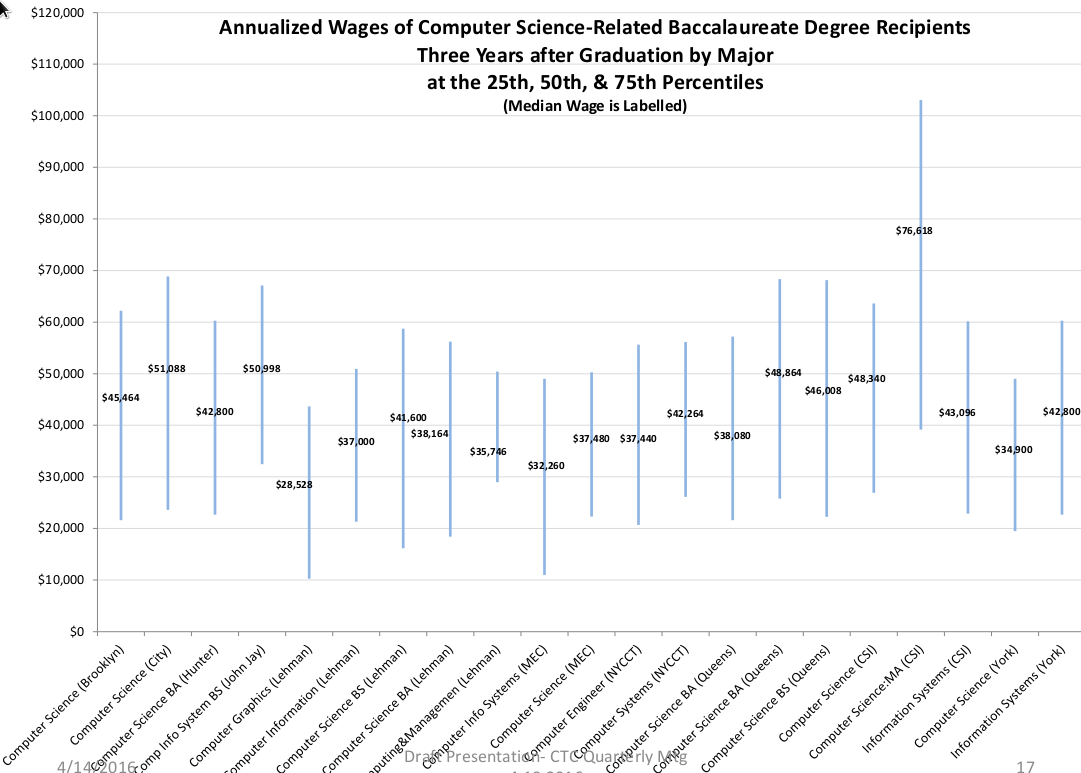
\includegraphics[width=.9\linewidth]{./images/salaryDist.png}
\end{center}
\end{frame}















\begin{frame}[label={sec:org20ac247}]{References}
\begin{itemize}
\item \href{http://www2.cuny.edu/wp-content/uploads/sites/4/page-assets/about/administration/offices/oira/institutional/surveys/SES\_Presentation\_EMC\_accessible.pdf}{CUNY Student Experience 2016}
\item \href{https://techcrunch.com/2015/08/20/new-york-citys-tech-industry-is-62-percent-white-60-percent-male/}{NYC Tech is 62\% White, 60\% male}
\item \href{https://nycfuture.org/data/nycs-tech-profile}{NYC Tech Profile}
\item \href{https://citylimits.org/2015/09/15/why-is-new-york-citys-growing-technology-sector-so-white/}{Why NYC's Growing Tech Sector is so White}
\item \href{http://www.crainsnewyork.com/article/20150706/BLOGS01/150709955/numbers-say-new-yorks-tech-boom-is-real}{Numbers say New York's tech boom is real}
\item \href{http://libertystreeteconomics.newyorkfed.org/2015/07/will-silicon-alley-be-the-next-silicon-valley.html\#.VZvrd-fDFB8}{Will Silicon Alley Be the Next Silicon Valley?}
\item \href{https://www.osc.state.ny.us/osdc/rpt4-2018.pdf}{The Technology Sector in New York City}
\item \href{http://worldpopulationreview.com/us-cities/new-york-city-population/}{NYC Population}
\item \href{http://www1.nyc.gov/office-of-the-mayor/news/677-17/de-blasio-administration-new-initiative-double-number-graduates-tech}{CUNY 2x Initiative}
\item \href{https://sites.google.com/a/lclark.edu/drake/courses/pls}{Peter Drake's Prog Lang Course Materials}
\item \url{http://learnyouahaskell.com/}
\end{itemize}
\end{frame}
\end{document}